\chapter{Результаты}
В ходе выполнения лабораторной работы оказалось, что в ЛР5 была допущена ошибка, в формуле случайной величины Эрланга, которая была исправлена, а также дополнена для сравнения. На рисунках \ref{p2}--\ref{p7} можно увидеть совпадение результатов работ программ на C$\#$ и GPSS:

\begin{figure}[!h]
	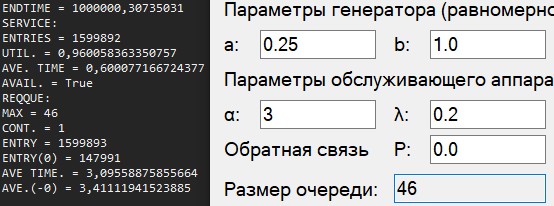
\includegraphics[width=1\linewidth]{inc/img/2.png}
	\caption{Результат программы на C$\#$ без обратной связи}
	\label{p2}
\end{figure}

\begin{figure}[!h]
	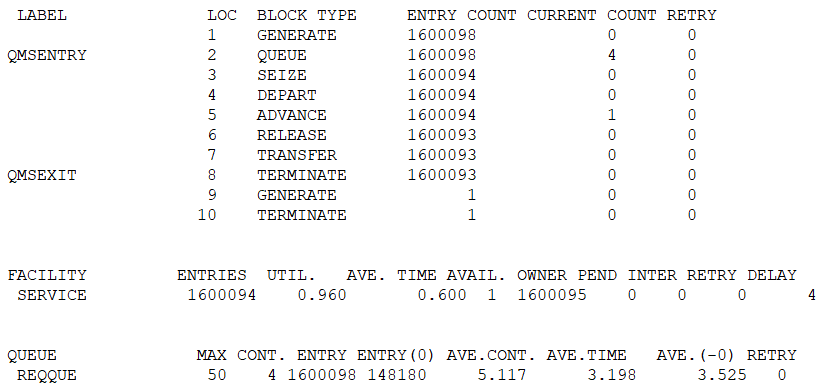
\includegraphics[width=1\linewidth]{inc/img/3.png}
	\caption {Результат программы на GPSS без обратной связи}
	\label{p3}
\end{figure}

\newpage
\begin{figure}[!h]
	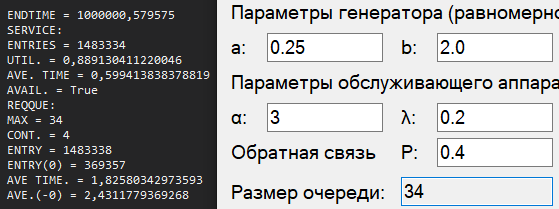
\includegraphics[width=1\linewidth]{inc/img/4.png}
	\caption{Результат программы на C$\#$ c обратной связью}
	\label{p4}
\end{figure}

\begin{figure}[!h]
	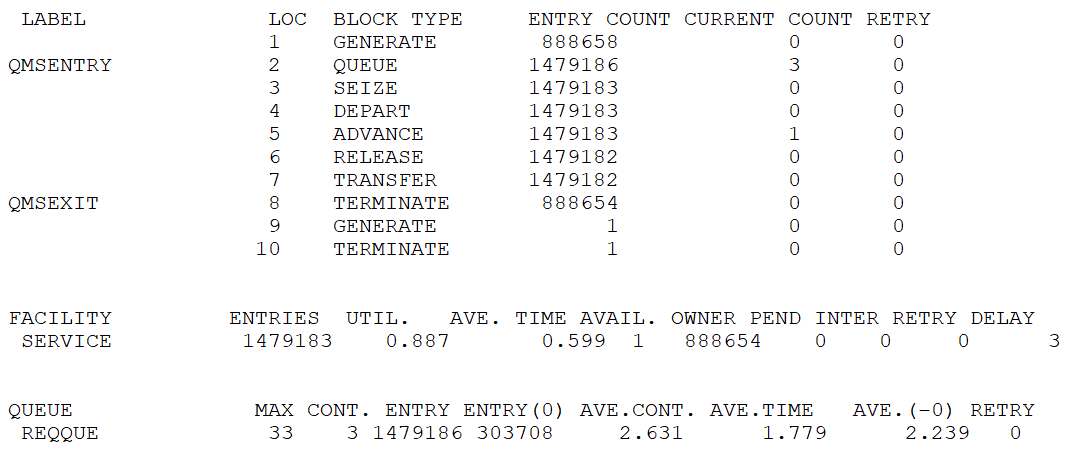
\includegraphics[width=1\linewidth]{inc/img/5.png}
	\caption{Результат программы на GPSS c обратной связью}
	\label{p5}
\end{figure}

\newpage
\begin{figure}[!h]
	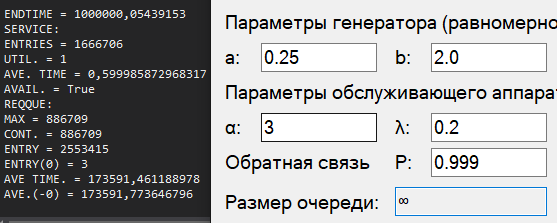
\includegraphics[width=1\linewidth]{inc/img/6.png}
	\caption{Результат программы на C$\#$ c обратной связью = 1}
	\label{p6}
\end{figure}

\begin{figure}[!h]
	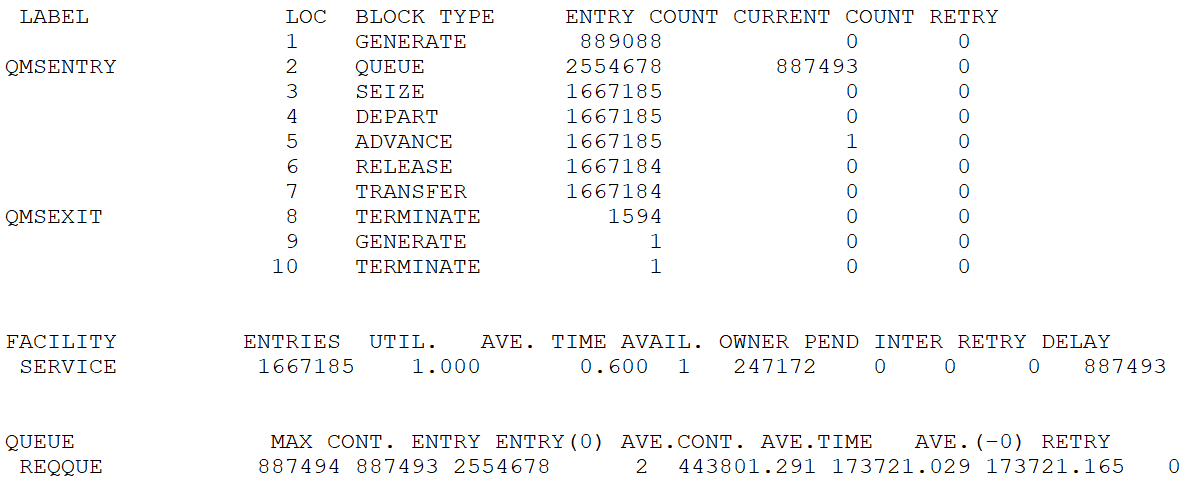
\includegraphics[width=1\linewidth]{inc/img/7.png}
	\caption{Результат программы на GPSS c обратной связью = 1}
	\label{p7}
\end{figure}

\newpage
На рисунке \ref{p1} изображен график построенный средствами GPSS, который отображает зависимость максимального размера очереди от времени моделирования с параметрами $a = 0.25, b = 1.0, \alpha = 3, \lambda = 0.2$:
\newline

\begin{figure}[!h]
	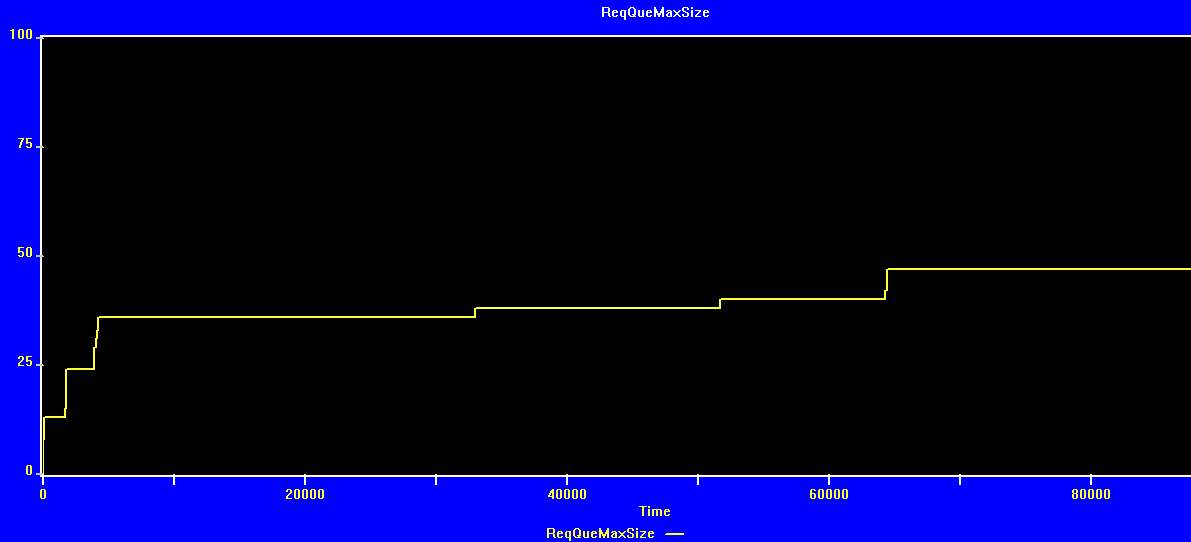
\includegraphics[width=1\linewidth]{inc/img/1.png}
	\caption{Зависимость максимального размера очереди от времени моделирования}
	\label{p1}
\end{figure}

А на рисунке \ref{p8} можно увидеть гистограмму отображающую статистическое распределение выборки времени ожидания: 

\begin{figure}[!h]
	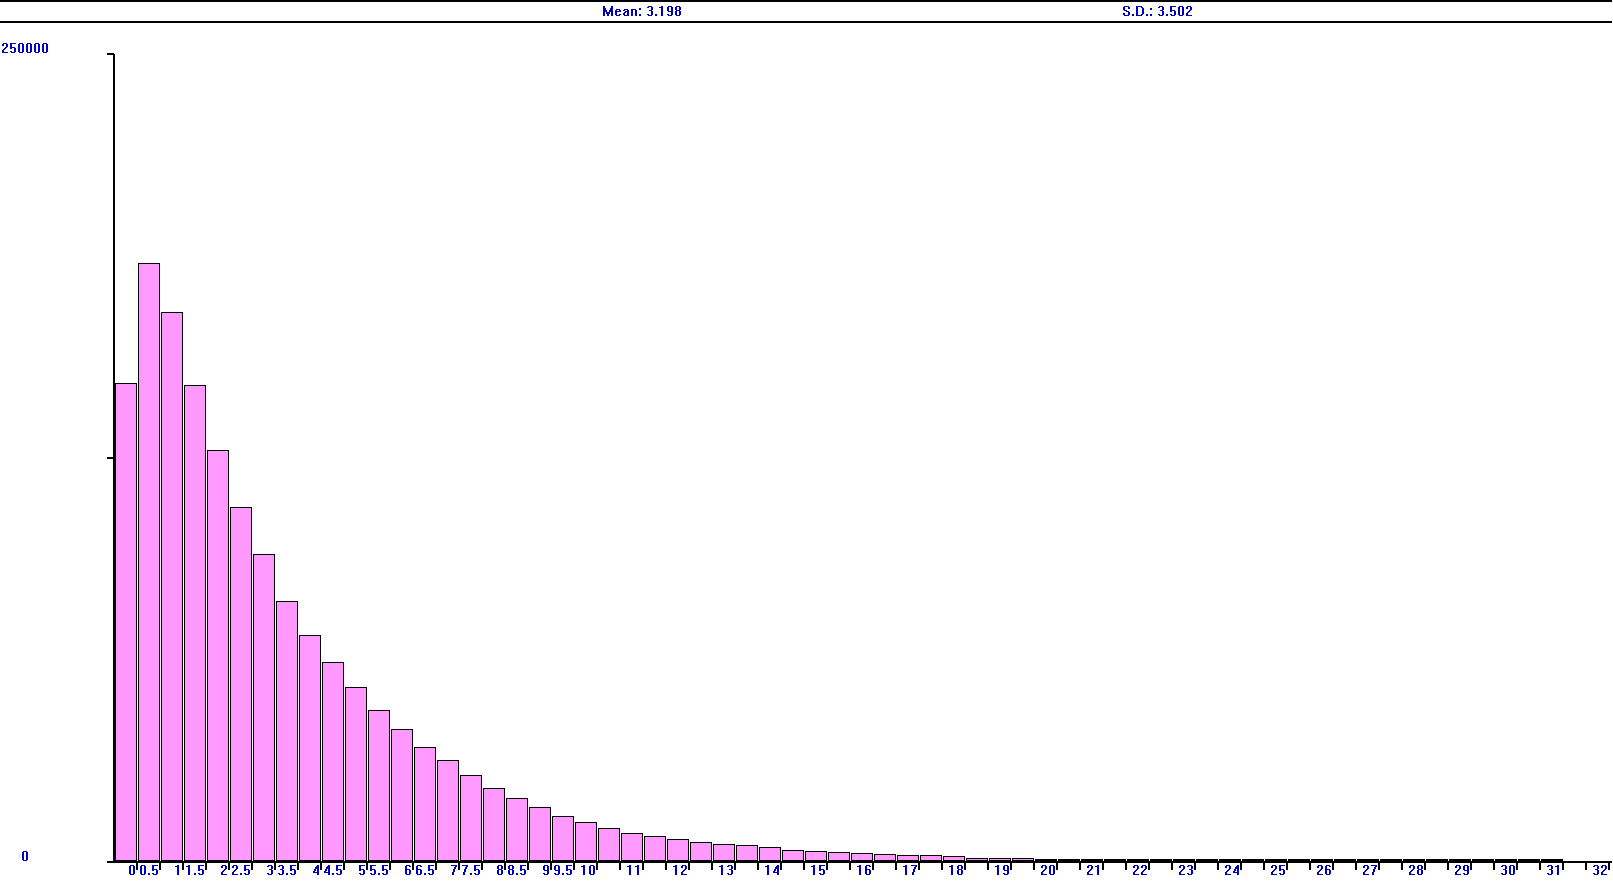
\includegraphics[width=1\linewidth]{inc/img/8.png}
	\caption{Статистическое распределение выборки времени ожидания}
	\label{p8}
\end{figure}
